Let
\begin{align}
\vec{A} = \myvec
{
-1 \\
 2\\
},
\vec{C} = 
\myvec
{
3\\
2\\
}
\end{align}
The given square is available in \figref{fig:7/4/4/4Fig1}.
\begin{figure}[!ht]
	\begin{center} 
	    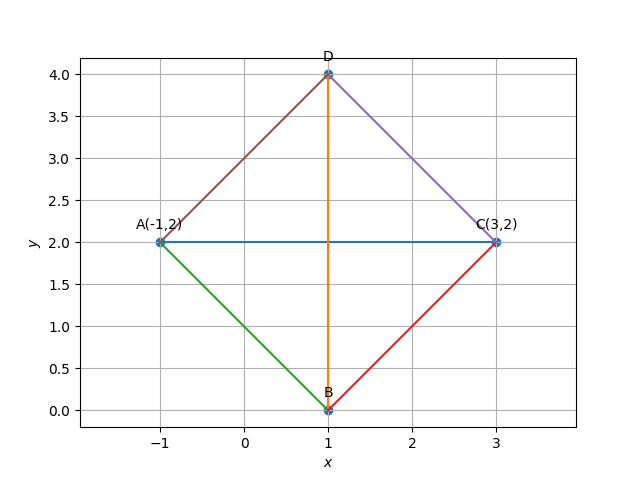
\includegraphics[width=\columnwidth]{chapters/10/7/4/4/figs/square}
	\end{center}
\caption{}
\label{fig:7/4/4/4Fig1}
\end{figure}
Shifting $\vec{A}$ to origin with reference to \figref{fig:7/4/4/4Fig2},
\begin{align}
\vec{A}_1 =
\myvec{
0 \\
0\\
},
\vec{C}_1 = \vec{C}-\vec{A} = 
\myvec{
4 \\
0\\
}
\end{align}
\begin{figure}[!h]
	\begin{center} 
	    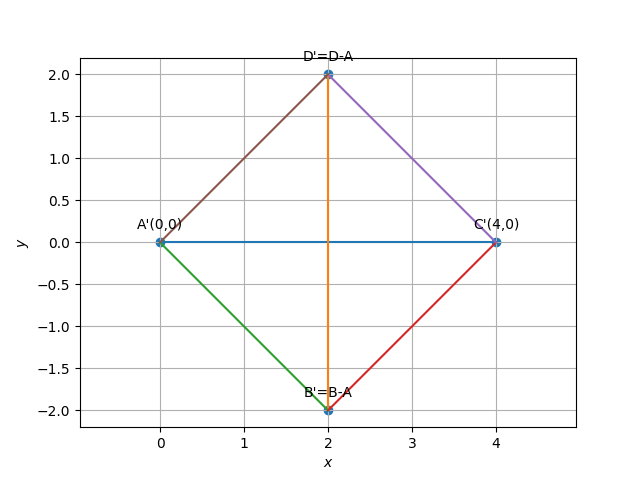
\includegraphics[width=\columnwidth]{chapters/10/7/4/4/figs/square1}
	\end{center}
\caption{}
\label{fig:7/4/4/4Fig2}
\end{figure}
Since
\begin{align}
\vec{C} - \vec{A} = \myvec{
4\\
0
} \equiv 
\myvec{
1\\
0
},\,
\theta= 0\degree
\end{align}
		where
$\theta$ is the angle made by $AC$ with the x-axis.
Considering the rotation matrix 
\begin{align}
\vec{P} =
\myvec{
\cos\brak{\frac{\pi}{4}-\theta} & -\sin\brak{\frac{\pi}{4}-\theta} \\
\sin\brak{\frac{\pi}{4}-\theta} & \cos\brak{\frac{\pi}{4}-\theta} 
}
\end{align}
\begin{figure}[!h]
	\begin{center} 
	    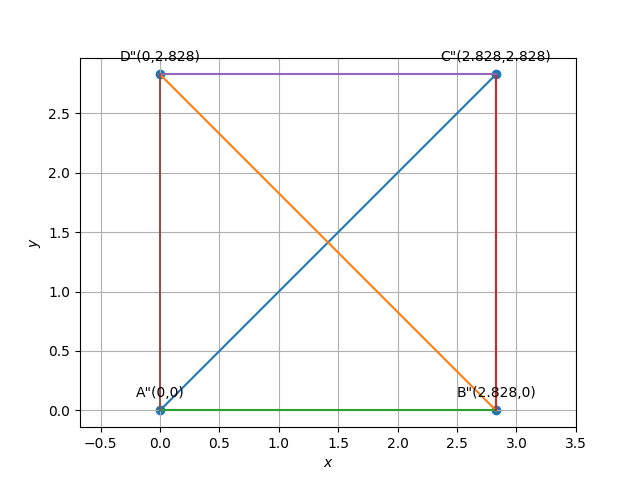
\includegraphics[width=\columnwidth]{chapters/10/7/4/4/figs/square2}
	\end{center}
\caption{}
\label{fig:7/4/4/4Fig3}
\end{figure}
From 
\figref{fig:7/4/4/4Fig3},
\begin{align}
	\vec{C}_2 &= \vec{P} (\vec{C}-\vec{A}) 
	\\
\label{eq:7/4/4/4bp}
	\vec{B}_2 &= \myvec{\vec{e}_1 & \vec{0}}\vec{C}_2
	\\
\label{eq:7/4/4/4dp}
	\vec{D}_2 &= \myvec{ \vec{0} & \vec{e}_2}\vec{C}_2
\end{align}
Now, 
\begin{align}
\label{eq:7/4/4/4b}
	\vec{B} = \vec{P}^{\top}\vec{B}_2+\vec{A}
	\\
\label{eq:7/4/4/4d}
	\vec{D} = \vec{P}^{\top}\vec{D}_2+\vec{A}
\end{align}
by reversing the process of translation and rotation.  Thus, 
from
\eqref{eq:7/4/4/4b}
\eqref{eq:7/4/4/4bp},
\eqref{eq:7/4/4/4d}
and
\eqref{eq:7/4/4/4dp}
\begin{align}
	\vec{B} = \vec{P}^{\top}\myvec{\vec{e}_1 & \vec{0}}\vec{P} (\vec{C}-\vec{A}) +\vec{A}
	\\
	\vec{D} = \vec{P}^{\top}\myvec{\vec{0} & \vec{e}_2  }\vec{P} (\vec{C}-\vec{A}) +\vec{A}
\end{align}
yielding
		\begin{align}
\vec{B}=
\myvec{
1\\
0
},
\vec{D}
\myvec{
1\\
4
}.
		\end{align}
